%!LW recipe=latexmk (XeLaTeX)
\documentclass[12pt,hyperref,a4paper,UTF8]{ctexart}
\usepackage{SJTUReport}
\usepackage{booktabs} % 三线表
\usepackage{amsmath}
\usepackage{amssymb} 

%%-------------------------------正文开始---------------------------%%
\begin{document}

% %-----------------------封面--------------------%%
\cover

%------------------摘要-------------%%
\newpage
\begin{abstract}

在此填写摘要内容

\end{abstract}
\newpage

\thispagestyle{empty} % 首页不显示页码

%%--------------------------目录页------------------------%%
\newpage
\tableofcontents

%%------------------------正文页从这里开始-------------------%
\newpage

%可选择这里也放一个标题
\begin{center}
   \title{ \Huge \textbf{{考虑异质用户的高速公路换电站运营MPC-RL分层协同优化}}}
\end{center}




\section{Introduction}
随着电动汽车在高速公路中长距离出行场景中的普及，沿线换电站的运营能力逐渐成为影响用户出行可靠性与系统运行效率的关键因素。相比传统充电方式，换电模式能够显著缩短车辆补能时间，但其运营过程同时受到用户到达需求、电池库存状态、站内充电过程以及电价变化等因素影响。特别是在高速公路场景中，用户行驶路径具有明显的方向性和连续性，不同车辆的初始 SOC 存在差异，导致其可达站点、可行换电路径以及对站内满电电池的占用情况均不相同。因此，高速公路换电站运营本质上是一个具有时空耦合、库存动态演化和不确定需求特征的序贯决策问题。

在实际运营中，系统中存在两类异质用户：预约用户和随机到达用户。预约用户通常提前给出出发时间、OD 路径和初始 SOC 信息，运营者需要在用户出行前对其换电站点进行合理分配，以提高服务确定性；随机用户的到达则具有更强的不确定性，运营者需要根据当前电池库存和未来需求预期决定是否服务。若仅基于当前满电电池数量进行局部决策，可能导致某些站点的满电电池被提前消耗，从而影响后续预约用户的服务可靠性；若过度保守地保留库存，又会降低随机用户服务量和系统收益。因此，如何在预约用户优先服务、随机用户灵活接纳以及电池充电调度之间进行协调，是高速公路换电网络运营中的核心问题。

针对上述问题，本文构建 MPC-RL 分层协同优化框架。换电站运营中存在两类性质不同但相互耦合的决策：一类是用户服务分配决策，包括预约用户路径指派和随机用户服务量决策；另一类是充电功率决策，即不同站点、不同 SOC 电池在不同时段的充电功率安排。本文采用模型预测控制（Model Predictive Control, MPC）处理用户服务分配问题，主要原因在于该问题包含 SOC 相关可达性、网络流平衡、满电电池可用性、预约用户优先级和库存非负性等硬约束，且可行动作集合会随 OD、初始 SOC、历史已出发车辆和站点库存动态变化。若直接采用 RL 进行用户指派，需要设计高维组合动作空间并处理大量动态 action masking，训练稳定性和可行性保障均较困难。相比之下，MPC 能够在滚动预测时域内显式刻画上述约束，并给出可解释、可执行的服务分配方案。

另一方面，充电功率决策虽然也可由 MPC 直接优化，但其影响具有明显的跨时段累积性：当前充电功率不仅决定当前充电成本，还会改变未来各站点不同 SOC 电池分布、满电电池供给能力和后续用户服务水平。由于充电功率动作维度相对固定，本文采用强化学习（Reinforcement Learning, RL）学习充电功率控制策略，使其能够在长期交互过程中根据需求、电价和库存状态自适应调整充电行为。如\autoref{fig:MPC-RL}所示，RL 层输出充电功率决策并影响电池状态转移，MPC 层在给定功率策略下优化预约用户和随机用户的服务分配。

进一步地，本文利用 RL critic 提供预测时域之外的长期价值信息，以缓解有限预测时域导致的末端效应。传统 MPC 通常通过设置固定终端库存下界避免时域末端过度消耗满电电池，但该方法只能粗略限制末端满电电池数量，难以区分不同站点、不同 SOC 电池在未来需求和电价环境下的长期价值。本文在 RL 训练过程中学习状态价值函数，并在每轮 MPC 求解前计算 critic 对终端库存的梯度，将其作为终端库存的长期边际价值系数。由此，RL 学到的长期价值被转化为 MPC 目标函数中的线性终端价值项，而无需将非线性神经网络直接嵌入优化模型。

因此，本文提出的 MPC-RL 框架并非将两类方法简单拼接，而是基于决策属性进行分层：MPC 负责处理强约束、组合结构明显且需要可解释性的用户服务分配问题；RL 负责学习具有长期影响的充电功率策略，并通过 critic 向 MPC 提供终端库存价值信息。二者通过电池库存状态、充电功率决策和终端价值项相互连接，从而在保证预约用户服务优先级和运营约束可行性的同时，使有限时域 MPC 能够近似感知预测时域之外的长期影响。

本文其余部分安排如下：第 2 节介绍 MPC 优化模型，包括时域设置、变量定义、SOC-wise expanded network 建模方法以及数学规划模型；第 3 节介绍 RL formulation，包括马尔可夫决策过程的建立和所选 RL 算法；第 4 节和第 5 节分别预留实验分析和结论部分。

\begin{figure}[!htbp]
    \centering
    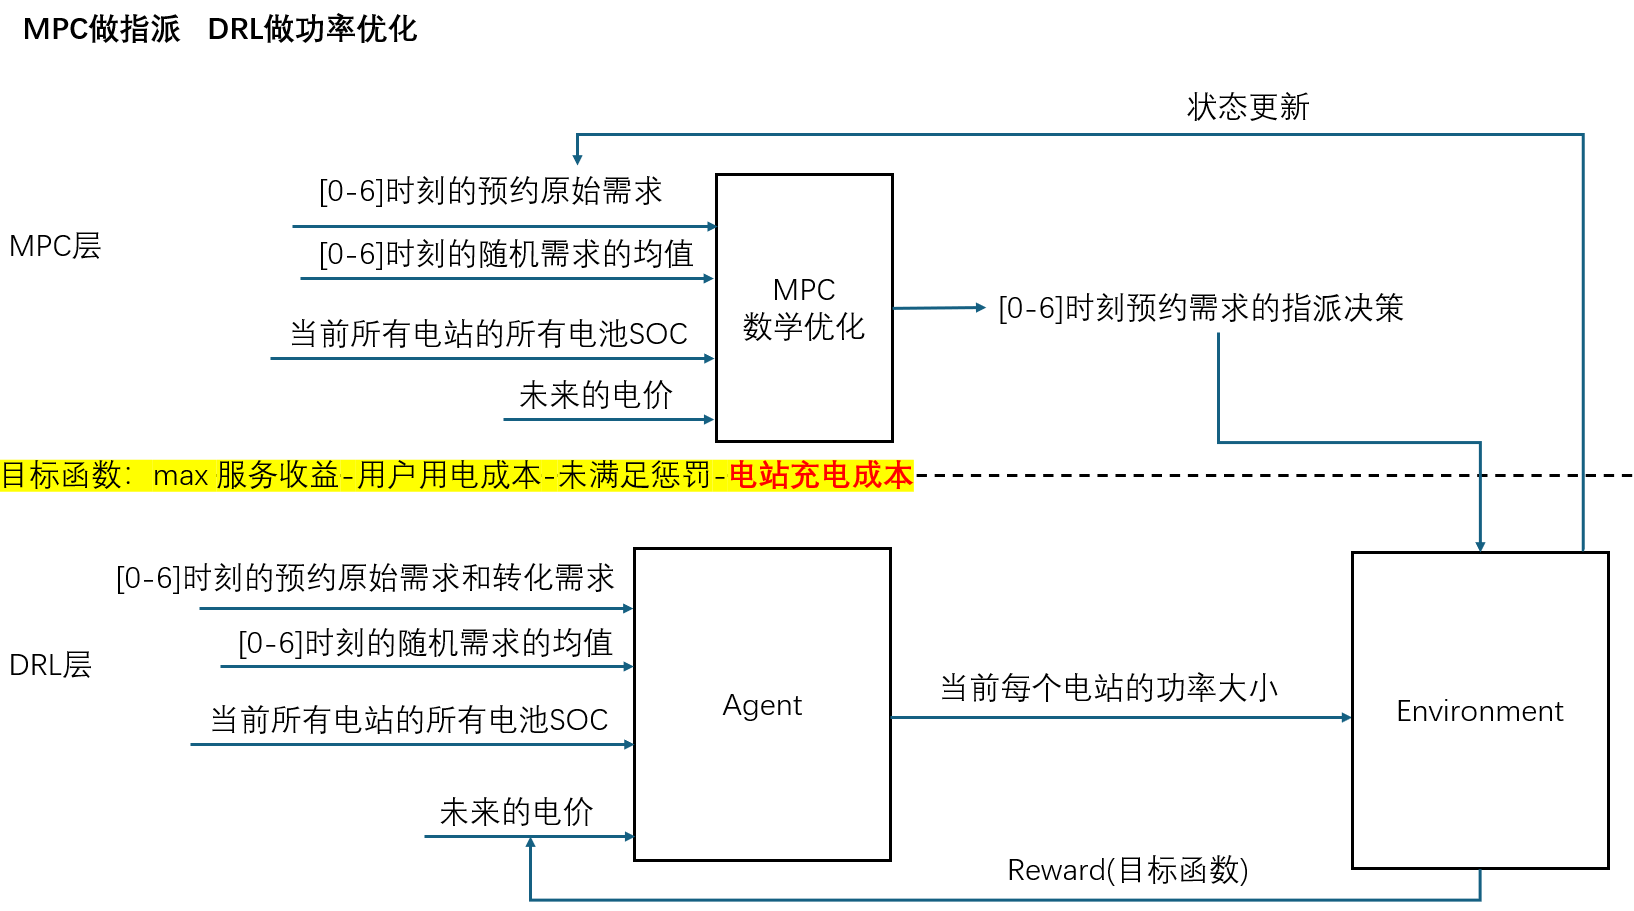
\includegraphics[width =1.0\textwidth]{figures/MPC-RL.png}
    \caption{MPC-RL协同优化框架}
    \label{fig:MPC-RL}
\end{figure}

\section{MPC Formulation}
\subsection{时域设置}

\begin{figure}[!htbp]
    \centering
    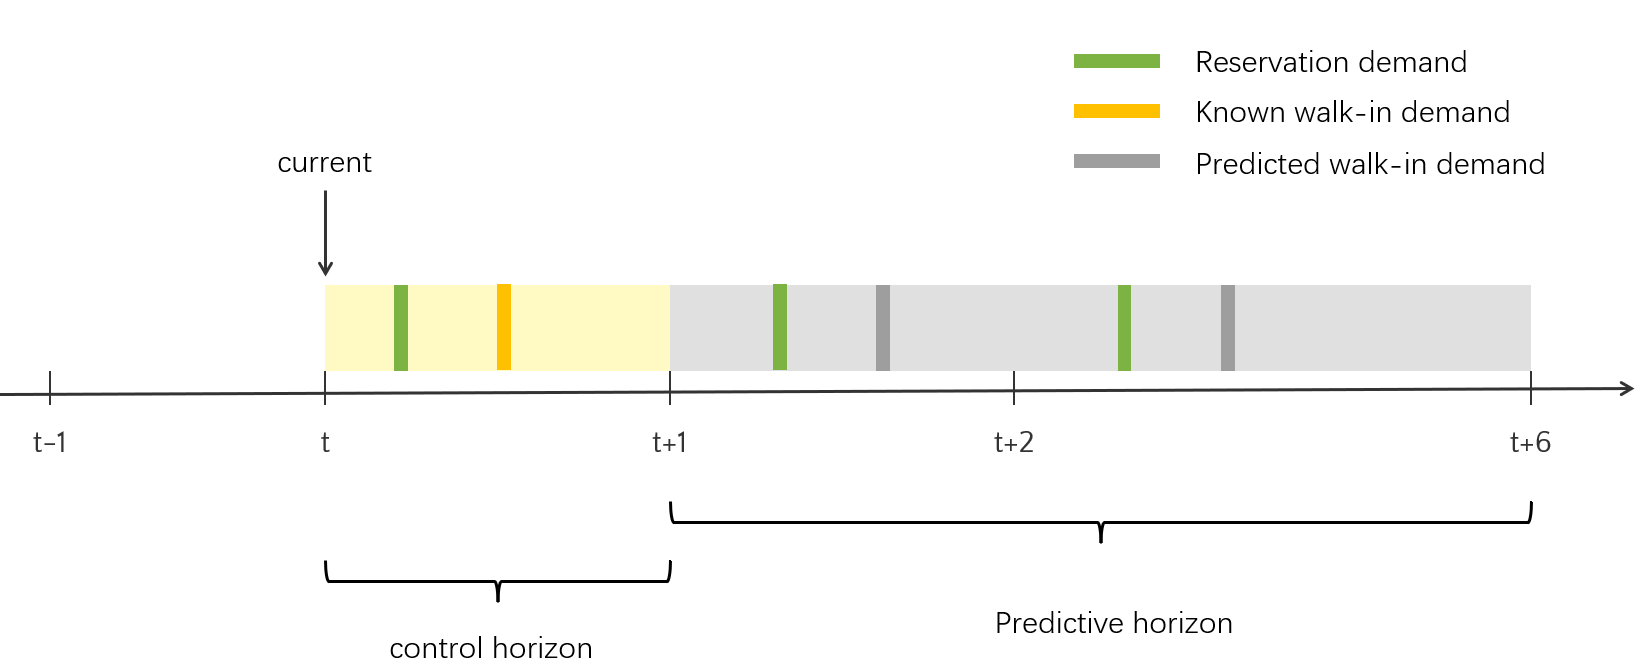
\includegraphics[width =1.0\textwidth]{figures/time_line.png}
    \caption{Rolling Horizon}
    \label{fig:Rolling Horizon}
\end{figure}

本文采用滚动时域思想刻画换电站运营中的动态决策过程。设当前决策时刻为 $t_0$，预测时域长度为 $H$。在每一轮 MPC 中，系统根据当前观测到的电池 SOC 库存、已知预约需求、随机需求预测、电价信息以及 RL 层给定的充电功率策略，求解未来 $H$ 个时段内的用户服务分配问题。求解完成后，仅执行当前时段的决策，并在进入下一时刻后根据新的系统状态重新构造并求解 MPC 问题。

为区分服务决策和库存状态，本文设决策时段集合为 $\mathcal{T}=\{1,\ldots,H\}$，电池库存状态时点集合为 $\mathcal{T}^{w}=\{0,1,\ldots,H\}$。其中，预约用户服务变量 $y_{A,i,j}^{n,p,t}$ 和随机用户服务变量 $y_R^{n,i,t}$ 定义在决策时段 $t\in\mathcal{T}$ 上；电池库存变量 $w_{n,i,t}$ 定义在状态时点 $t\in\mathcal{T}^{w}$ 上。该设置使得库存状态可以由初始时点 $0$ 逐期递推至预测时域末端 $H$，从而为终端库存价值的刻画提供基础。

在预约用户服务方面，本文不强制要求所有预约需求均被服务，而是通过较高的未满足预约需求惩罚和预约用户优先服务约束体现预约用户的服务优先级。这种处理方式可以避免在需求超过系统服务能力时造成模型不可行，同时通过惩罚项引导模型尽可能满足预约需求。若实际运营中要求所有成功预约用户必须得到服务，则可在预约接受阶段额外设置容量控制机制；本文重点关注给定预约需求下的滚动服务分配与电池库存协同优化。

\subsection{变量列表}

本文使用的变量如\autoref{tab:notation}所示。

\begin{table}[!htbp]
  \centering
  \caption{Notation table}
  \label{tab:notation}
  \footnotesize
  \setlength{\tabcolsep}{1pt}
  \renewcommand{\arraystretch}{0.85}
  \begin{tabular}{@{}lp{13cm}@{}}
    \toprule
    \textbf{Notation} & \textbf{Description} \\
    \midrule
    \multicolumn{2}{l}{\textit{Sets and Indices}} \\
    $\mathcal{P}$ & Set of O-D pairs, indexed by $p$\\
    $\mathcal{T}$ & Set of decision time periods in predictive horizon, $\mathcal{T}:=\{1,\dots,H\}$, indexed by $t$ \\
    $\mathcal{T}^{w}$ & Set of battery inventory state time points, $\mathcal{T}^{w}:=\{0,1,\dots,H\}$, indexed by $t$ \\
    $\mathcal{N}$ & Set of charging state of batteries, $\mathcal{N}:=\{0,\dots,N\}$, indexed by $n$\\
    $\mathcal{B}$ & Set of batteries in each station, indexed by $b$ \\
    $\mathcal{S}^p$ & Set of intermediate BSSs passed through O-D pair $p$, indexed by $i, j$ \\
    $\mathcal{S}$ & Set of all BSSs in the system, $\mathcal{S}$:=$\bigcup_{p \in \mathcal{P}}\mathcal{S}^p$\\
    $\mathcal{V}^p$ & Set of nodes consisting of origin $o^p$, destination $d^p$, and all BSS $\mathcal{S}^p$ on the path of O-D pair $p$ \\  
    $\mathcal{A}^{n,p}$ & Set of arcs in battery swapping network for original state $n$, O-D pair $p$ \\
    $\mathcal{G}^{n,p}$ & Directed graph for original state $n$, O-D pair $p$, $\mathcal{G}^{n,p}:=(\mathcal{V}^p,\mathcal{A}^{n,p})$ \\
    $Path^p$ & Set of all possible paths from origin to destination for O-D pair $p$ \\
    \midrule
    \multicolumn{2}{l}{\textit{Parameters}} \\
    % $s^q$ & Origin node of demand flow $q$ \\
    % $r^q$ & Destination node of demand flow $q$ \\
    % $H$ & Number of decision periods in the predictive horizon \\
    $R$ & Driving range \\
    % R^L$ & Driving range of long-range battery (km) \\
    % $N^b$ & Number of time periods required to fully charge a battery of type $b$\\
    % $N^l$ & Number of time periods required to fully charge a long-range battery \\
    % $M_i$ & Number of available charging slots at station $i$ \\
    $\tau_{p,i,t}$ & The travel time of the EV departing at time $t$ arriving to station $i$ for O-D pair $p$\\
    $\tau_{p,max}$ & The maximum travel time of the EV for O-D pair $p$\\
    $P_{b,i,t}$ & Charging power of each battery $b$ in station $i$ in time period $t$\\
    $e_{i,t}$ & Electricity price at station $i$ in time period $t$\\
    $s_{i,t}$ & Service fee for battery swap of type $b$ at station $i$ in time period $t$\\
    $v^{n,p}_{i,j}$ & The amount of electricity consumed by an appointed EV with an initial charging state $n$ from station $i$ to $j$ for O-D pair $p$\\
    $v^{n}_{i}$ & The amount of electricity consumed by a walk-in EV with an initial charging state $n$ arriving at station $i$\\
    % $SOC_{b,i,t}$ & soc of battery $b$ at station $i$ in time period $t$ \\ 
    % $P_t^L$ & Service fee for long-range battery swap at time $t\in\mathcal{T}$\\
    % $P^C$ & Compensation for long-range customers swapping to standard-range battery\\
    % $c^b$ & Unit temporary configuration cost of batteries of type $b$ \\
    % $c^L$ & Unit cost of long-range battery (currency) \\
    $x_i^b$ & Initial number of batteries at station $i$ \\
    % $\hat{x}_i^L$ & Initial number of long-range batteries at station $i$ \\
    % $\bar{I}$ & Maximum battery inventory limit at each station \\
    $\alpha$ & Penalty cost per unit of unsatisfied reservation demand\\
    % $\beta$ & Weight coefficient of the RL-enhanced terminal value in the MPC objective \\
    % $\gamma$ & Discount factor used in RL critic training \\
    % $V_{\theta}(s)$ & RL critic/value function parameterized by $\theta$, which approximates the long-term return from system state $s$ \\
    $\bar{s}_{t+H}$ & Reference terminal state used to linearize the RL critic before solving the MPC problem \\
    $\lambda_{i,n,t}$ & Marginal terminal value of one additional battery with SOC state $n$ at station $i$, computed from the gradient of $V_{\theta}(s)$ at $\bar{s}_{t+H}$ \\
    $f_A^{n,p,t}$ & Reservation demand volume of EVs in original state $n$ for O-D pair $p$ at time $t$ \\
    $f_{R}^{n,i,t}$ & Random demand volume of EVs in original state $n$ at station $i$ in time period $t$ \\
    $\bar{y}_{A,i,j}^{n,p,k}$ & Historical service volume of reservation flows on arc $(i,j)$ that departed before the current predictive horizon, indexed by $k\in\{-\tau_{p,max},\dots,0\}$ \\
    $\bar{w}_{n,i,0}$ & Initial number of batteries in charging state $n$ at station $i$ \\
    $\underline{w}_{N,i}$ & Minimum number of fully charged batteries retained at station $i$ at the end of the predictive horizon \\
    % $\Phi^{\mathrm{RL}}_t$ & Linear terminal value term provided by the RL critic at decision time $t$ \\
    $s_t$ & Markov state observed by the RL agent at decision time $t$ \\
    $a_t$ & RL action vector, representing the charging power decision used by the MPC layer and the environment \\
    $\pi_{\phi}(a_t\mid s_t)$ & Stochastic charging power policy parameterized by $\phi$ \\
    $r_t$ & Immediate reward in the RL formulation, defined consistently with the realized operating profit of the system \\
    % $f_{\xi}^{L,q,t}$ & Demand volume of long-range EVs for flow $q$ at time $t$ under scenario $\xi$ \\
    \midrule
    \multicolumn{2}{l}{\textit{Variables}} \\
    % $x_i^b$ & Number of batteries of type $b$ allocated at station $i$ \\
    % $x_i^L$ & Number of long-range batteries allocated at station $i$ \\
    $y_{A,i,j}^{n,p,t}$ & Service volume of demand volume $f_{A}^{n,p,t}$ on arc $(i,j) \in A^{n,p}$, $t\in\mathcal{T}$ \\
    $y_{R}^{n,i,t}$ & Service volume of random demand volume $f_{R}^{n,i,t}$, $t\in\mathcal{T}$\\
    % $y_{i,j}^{L,q,t}$ & Service flow volume of long-range demand $f^{L,q,t}$ on arc $(i,j) \in A^{L,q}$ \\
    % $\hat{y}_{i,j}^{b,q,t}$ & Service volume of demand volume $f_{\xi}^{b,q,t}$ on arc $(i,j) \in A^{\bar{b},q}$, where $\bar{b}$ represents another battery type \\
    % $\hat{y}_{i,j}^{L,q,t}$ & Service flow volume of long-range demand $f^{L,q,t}$ on arc $(i,j) \in A^{S,q}$ (flexible swap) \\
    $w_{n,i,t}$ & Number of batteries in charging state $n$ at station $i$ at inventory state time point $t\in\mathcal{T}^{w}$ \\
    % $w_{t,n}^{l,i}$ & Number of long-range batteries at station $i$ that have been charged for $n$ periods at time $t$ \\
    % $z_{t,n}^{b,i}$ & Number of stage $n$ batteries of type $b$ at station $i$ being charged at time $t$. \\
    % $z_{t,n}^{l,i}$ & Number of long-range batteries at station $i$ being charged during period $t$ that have been charged for $n$ periods \\
    \bottomrule
  \end{tabular}
\end{table}

\subsection{SOC-wise expanded network}

高速公路换电场景中的预约用户具有明确的 OD 路径和初始 SOC。由于初始 SOC 不同，同一 OD 对上的用户可达站点集合和可行换电路径可能不同。为刻画这种 SOC 相关的路径可行性，本文在传统 expanded network 的基础上构建 SOC-wise expanded network。该建模方法针对每一个 OD 对 $p\in\mathcal{P}$ 和每一个初始 SOC 状态 $n\in\mathcal{N}$，分别构造一个有向网络 $\mathcal{G}^{n,p}=(\mathcal{V}^{p},\mathcal{A}^{n,p})$。

在网络 $\mathcal{G}^{n,p}$ 中，节点集合 $\mathcal{V}^{p}$ 包括 OD 对 $p$ 的起点 $o^p$、终点 $d^p$ 以及该路径上可经过的所有中间换电站 $\mathcal{S}^{p}$。弧集合 $\mathcal{A}^{n,p}$ 用于表示在初始 SOC 为 $n$ 的条件下，用户从一个节点行驶到另一个节点并完成后续换电服务的可行连接。具体而言，若车辆在给定 SOC 状态下能够从节点 $i$ 行驶到节点 $j$，且该连接符合高速公路路径方向和最大行驶里程约束，则弧 $(i,j)$ 被加入 $\mathcal{A}^{n,p}$。因此，随着初始 SOC $n$ 的变化，网络中的可行弧集合也会发生变化。

该网络建模方式具有两个作用。第一，它将用户初始 SOC 对可达站点和换电路径的影响显式嵌入网络结构，使得不可行的站点选择不会进入优化模型。第二，它使预约用户指派问题可以表示为网络流决策：预约需求 $f_A^{n,p,t}$ 从起点 $o^p$ 进入网络，服务变量 $y_{A,i,j}^{n,p,t}$ 表示该类需求在弧 $(i,j)\in\mathcal{A}^{n,p}$ 上的服务流量。通过流平衡约束，模型可以保证被服务的预约用户沿一条可行路径从起点移动到终点，并在路径上的换电站消耗满电电池、归还低 SOC 电池。

需要注意的是，SOC-wise expanded network 主要用于刻画预约用户的可行路径和站点指派。随机用户由于在换电站现场到达，本文不再为其构造 OD 网络，而是直接通过 $y_R^{n,i,t}$ 表示时段 $t$、站点 $i$、初始 SOC 为 $n$ 的随机用户服务量。预约用户和随机用户在电池库存层面相互耦合：两类用户服务均会消耗站内满电电池，并向站内归还不同 SOC 状态的电池。

\begin{figure}[!htbp]
    \centering
    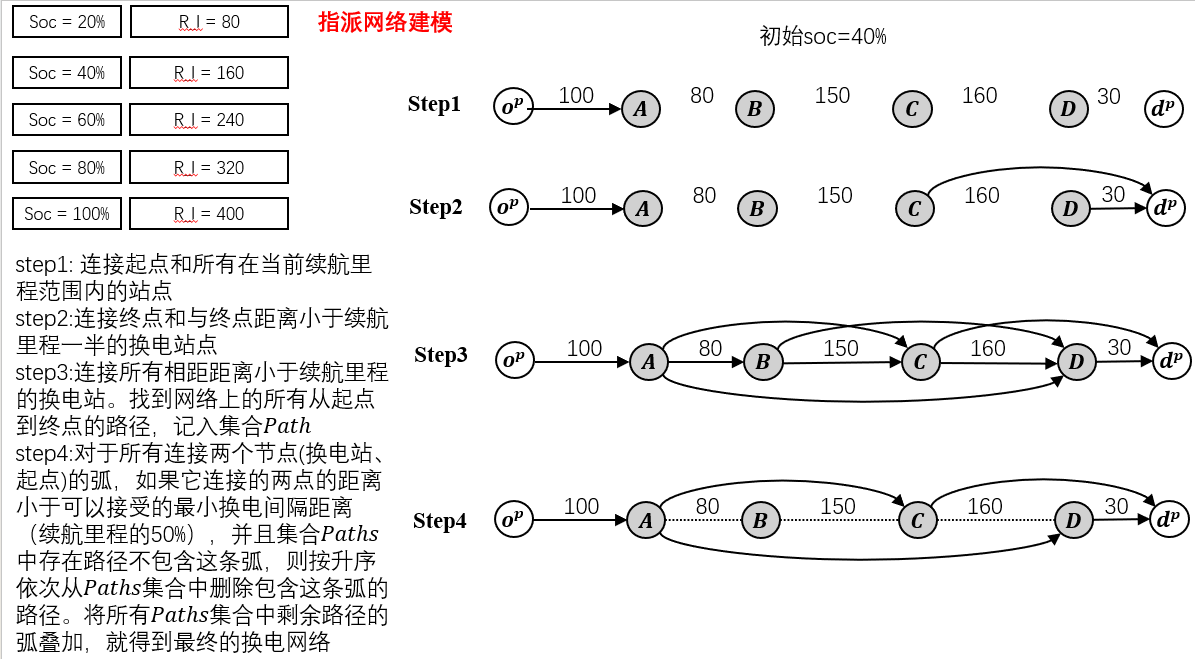
\includegraphics[width =1.0\textwidth]{figures/指派网络建模.png}
    \caption{指派网络建模}
    \label{fig:assignment network}
\end{figure}

\subsection{Mathematical model}

本节给出 MPC 层的数学规划模型。MPC 层的决策变量包括预约用户在 SOC-wise expanded network 上的服务流量 $y_{A,i,j}^{n,p,t}$、随机用户服务量 $y_R^{n,i,t}$ 以及各站点不同 SOC 电池库存 $w_{n,i,t}$。RL 层输出的充电功率 $P_{n,i,t}$ 在每轮 MPC 求解时作为外部给定参数进入电池状态转移和充电成本项。

\subsubsection{RL-enhanced terminal value within MPC}

有限预测时域 MPC 若仅优化预测时域内收益，可能在时域末端过度服务当前用户，从而留下对未来运营不利的库存结构。为此，本文将 RL critic 学到的长期价值信息嵌入 MPC 目标函数。RL 层学习状态价值函数
\begin{equation}
V_{\theta}(s_t)\approx
\mathbb{E}\left[\sum_{k=0}^{\infty}\gamma^k r_{t+k}\mid s_t\right],
\label{eq:critic_value}
\end{equation}
其中 $s_t$ 表示系统状态，$r_t$ 表示与运营目标一致的即时收益。

由于 $V_{\theta}(s)$ 通常由深度神经网络表示，若直接将其嵌入 MPC 会导致优化模型非线性且难以求解。因此，本文仅利用 critic 提取终端库存的局部边际价值。在每轮 MPC 求解前，首先构造参考终端状态 $\bar{s}_{t+H}$，该状态可由上一轮 MPC 的预测末端状态或给定 RL 功率策略下的名义滚动预测得到。然后在 $\bar{s}_{t+H}$ 处对 $V_{\theta}(s)$ 关于终端库存变量进行一阶线性化：
\begin{equation}
V_{\theta}(s_{t+H})
\approx
V_{\theta}(\bar{s}_{t+H})+
\sum_{i\in\mathcal{S}}\sum_{n\in\mathcal{N}}
\lambda_{i,n,t}\left(w_{n,i,H}-\bar{w}_{n,i,H}\right),
\label{eq:value_linearization}
\end{equation}
其中长期边际价值系数定义为
\begin{equation}
\lambda_{i,n,t}
=
\left.
\frac{\partial V_{\theta}(s)}{\partial w_{n,i}}
\right|_{s=\bar{s}_{t+H}},
\quad \forall i\in\mathcal{S},\ n\in\mathcal{N}.
\label{eq:marginal_value}
\end{equation}
式\eqref{eq:marginal_value} 表示在参考终端状态附近，预测时域末端站点 $i$ 多保留一块 SOC 为 $n$ 的电池所带来的长期收益边际贡献。由于 $V_{\theta}(\bar{s}_{t+H})$ 和 $\bar{w}_{n,i,H}$ 在 MPC 求解前均为常数，不影响优化决策，因此 MPC 目标函数中仅保留如下线性终端价值项：
\begin{equation}
\Phi^{\mathrm{RL}}_t
=
\sum_{i\in\mathcal{S}}\sum_{n\in\mathcal{N}}
\lambda_{i,n,t}w_{n,i,H}.
\label{eq:rl_terminal_value}
\end{equation}
在每次 MPC 求解时，$\lambda_{i,n,t}$ 均作为外部给定参数输入优化模型，因此终端价值项对决策变量 $w_{n,i,H}$ 保持线性，不会破坏原模型的可求解性。若 critic 的库存输入经过归一化处理，则需将梯度按照原始库存单位进行尺度还原后再作为 $\lambda_{i,n,t}$ 使用。

\subsubsection{Objective function}

目标函数为最大化预测时域内的服务收益，减去未满足预约需求惩罚和电站充电成本，并加入 RL critic 提供的线性终端价值：
\begin{equation}
\max \quad I-C_1-C_2+\beta\Phi^{\mathrm{RL}}_t.
\label{eq:objective}
\end{equation}

服务收益由预约用户和随机用户完成换电所产生的服务费构成：
\begin{equation}
I=\sum_{t \in \mathcal{T}}  \sum_{n \in \mathcal{N}} 
\left[  
\sum_{p \in \mathcal{P}} 
\sum_{\{(i,j) | (i,j) \in \mathcal{A}^{n,p}\}} 
\left ( y^{n,p,t+\tau_{p,i,t}}_{A,i,j}v^{n}_{i,j}s_{i,t+\tau_{p,i,t}} \right )
+\sum_{i \in \mathcal{S}} y_{R}^{n,i,t}v^n_is_{i,t}
\right].
\label{eq:income}
\end{equation}

未满足预约需求惩罚为
\begin{equation}
C_1 = \alpha \sum_{t\in \mathcal{T}} \sum_{p\in \mathcal{P}}  \sum_{n\in \mathcal{N}} 
\left[
f^{n,p,t}_A - \sum_{\{j | (o^p,j) \in \mathcal{A}^{n,p}\}} y^{n,p,t}_{A,o^p,j} \right].
\label{eq:penaltycost}
\end{equation}

电站充电成本为
\begin{equation}
C_2 = \sum_{t \in \mathcal{T}}  \sum_{n \in \mathcal{N}} \sum_{i \in \mathcal{S}}
\left[
w_{n,i,t}P_{n,i,t}e_{i,t}
\right].
\label{eq:chargingcost}
\end{equation}

\subsubsection{Constraints}

\paragraph{Flow conservation constraints.}
预约需求从起点进入 SOC-wise expanded network，且服务量不超过实际预约需求：
\begin{subequations}
\label{eq:flow}
\begin{gather}
\sum_{\{j| (o^p,j)\in \mathcal{A}^{n,p}\}}{y^{n,p,t}_{A,o^p,j}} \leq f^{n,p,t}_A,
\quad \forall p\in \mathcal{P},\ t\in \mathcal{T},\ n \in \mathcal{N},\label{eq:flow1}\\
\sum_{\{j| (i,j)\in \mathcal{A}^{n,p}\}}{y^{n,p,t}_{A,i,j}} =
\sum_{\{j| (j,i)\in \mathcal{A}^{n,p}\}}{y^{n,p,t}_{A,j,i}},
\quad \forall p\in \mathcal{P},\ t\in \mathcal{T},\ i\in \mathcal{S}^p,\ n\in\mathcal{N}.
\label{eq:flow2}
\end{gather}
\end{subequations}

\paragraph{Battery state transition constraints.}
对于 SOC 状态 $r<N$ 的电池，时刻 $t$、站点 $i$ 的库存由三部分组成：当前预测时域内到达并归还 SOC 为 $r$ 电池的预约用户、预测时域开始前已经出发但在当前时域内到达的历史预约用户、当前随机用户归还的 SOC 为 $r$ 电池，以及上一时刻经过充电后转移到 SOC $r$ 的站内电池。因此有
\begin{equation}
\begin{aligned}
w_{r,i,t}
=&
\sum_{p\in \mathcal{P}}
\sum_{n\in \mathcal{N}}
\sum_{\{j\mid (j,i)\in \mathcal{A}^{n,p}\}}
\sum_{\{k\in \mathcal{T}\mid k+\tau_{p,i,k}=t\}}
y^{n,p,k}_{A,j,i}
\mathbb{I}\!\left(N-v^{n,p}_{j,i}=r\right)
\\
&+
\sum_{p\in \mathcal{P}}
\sum_{n\in \mathcal{N}}
\sum_{\{j\mid (j,i)\in \mathcal{A}^{n,p}\}}
\sum_{\{k\in \{-\tau_{p,max},\ldots,0\}\mid k+\tau_{p,i,k}=t\}}
\bar{y}^{n,p,k}_{A,j,i}
\mathbb{I}\!\left(N-v^{n,p}_{j,i}=r\right)
\\
&+
y^{r,i,t}_{R}
+
\sum_{m\in \mathcal{N}}
w_{m,i,t-1}
\mathbb{I}\!\left(m+P_{m,i,t-1}=r\right),
\\
&\forall i\in \mathcal{S},\ r\in \mathcal{N}\setminus\{N\},\ t\in \mathcal{T}.
\end{aligned}
\label{eq:transition_nonfull}
\end{equation}

其中，$\mathbb{I}(N-v^{n,p}_{j,i}=r)$ 表示预约用户在电站 $i$ 退回的电池 SOC 为 $r$；$\mathbb{I}(m+P_{m,i,t-1}=r)$ 表示上一时刻 SOC 为 $m$ 的站内电池经过充电后在时刻 $t$ 变为 SOC $r$。

对于满电电池，时刻 $t$ 的库存等于上一时刻经充电达到满电的电池数量，减去当前时刻被预约用户和随机用户换走的满电电池数量：
\begin{equation}
\begin{aligned}
w_{N,i,t}
=&
\sum_{m\in \mathcal{N}}
w_{m,i,t-1}
\mathbb{I}\!\left(m+P_{m,i,t-1}=N\right)
\\
&-
\sum_{p\in \mathcal{P}}
\sum_{n\in \mathcal{N}}
\sum_{\{j\mid (i,j)\in \mathcal{A}^{n,p}\}}
\sum_{\{k\in \mathcal{T}\mid k+\tau_{p,i,k}=t\}}
y^{n,p,k}_{A,i,j}
\\
&-
\sum_{p\in \mathcal{P}}
\sum_{n\in \mathcal{N}}
\sum_{\{j\mid (i,j)\in \mathcal{A}^{n,p}\}}
\sum_{\{k\in \{-\tau_{p,max},\ldots,0\}\mid k+\tau_{p,i,k}=t\}}
\bar{y}^{n,p,k}_{A,i,j}
\\
&-
\sum_{n\in \mathcal{N}}
y^{n,i,t}_{R},
\\
&\forall i\in \mathcal{S},\ t\in \mathcal{T}.
\end{aligned}
\label{eq:transition_full}
\end{equation}

\paragraph{Swapping priority constraints.}
由于换电站仅向用户提供满电电池，时刻 $t$ 电站 $i$ 可用于换电的满电电池数量为上一时刻站内电池经过充电后达到满电状态的电池数量。预约用户具有优先服务权，随机用户只能使用预约用户换电后剩余的满电电池：
\begin{equation}
\begin{aligned}
\sum_{n\in \mathcal{N}} y^{n,i,t}_{R}
&\le
\biggl[
\sum_{m\in \mathcal{N}} w_{m,i,t-1}
\mathbf{1}\!\left(m+P_{m,i,t-1}=N\right) \\
&-
\sum_{p\in \mathcal{P}}
\sum_{n\in \mathcal{N}}
\sum_{\{j\mid (j,i)\in \mathcal{A}^{n,p}\}}
\sum_{\{k\in \mathcal{T}\mid k+\tau_{p,i,k}=t\}}
y^{n,p,k}_{A,j,i} \\
&-
\sum_{p\in \mathcal{P}}
\sum_{n\in \mathcal{N}}
\sum_{\{j\mid (j,i)\in \mathcal{A}^{n,p}\}}
\sum_{\{k\in \{-\tau_{p,\mathrm{max}},\ldots,0\}\mid k+\tau_{p,i,k}=t\}}
\bar{y}^{n,p,k}_{A,j,i}\biggr]^+,
\\
&\quad \forall i\in \mathcal{S},\ t\in \mathcal{T}.
\end{aligned}
\label{eq:priority}
\end{equation}

同时，随机用户服务量不得超过实际随机需求：
\begin{equation}
0\le y^{n,i,t}_{R}\le f^{n,i,t}_{R},
\qquad
\forall i\in \mathcal{S},\ n\in \mathcal{N},\ t\in \mathcal{T}.
\label{eq:random_bound}
\end{equation}

\paragraph{Boundary and integrality constraints.}
预测时域起点的电池 SOC 分布为已知初始状态：
\begin{equation}
w_{n,i,0}=\bar{w}_{n,i,0},
\quad \forall n\in \mathcal{N},\ i\in \mathcal{S}.
\label{eq:initial_inventory}
\end{equation}

所有服务量和电池库存变量均应满足非负性约束：
\begin{gather}
w_{n,i,t}\ge 0,
\quad \forall n\in \mathcal{N},\ i\in \mathcal{S},\ t\in \mathcal{T}^{w},
\label{eq:nonnegative_w}\\
y^{n,p,t}_{A,i,j}\ge 0,
\quad \forall p\in \mathcal{P},\ n\in \mathcal{N},\ t\in \mathcal{T},\ (i,j)\in \mathcal{A}^{n,p},
\label{eq:nonnegative_a}\\
y^{n,i,t}_{R}\ge 0,
\quad \forall n\in \mathcal{N},\ i\in \mathcal{S},\ t\in \mathcal{T}.
\label{eq:nonnegative_r}
\end{gather}

若需求量和电池数量均以整数计，则进一步有
\begin{equation}
w_{n,i,t}\in \mathbb{Z}_{+},\quad
 y^{n,p,t}_{A,i,j}\in \mathbb{Z}_{+},\quad
 y^{n,i,t}_{R}\in \mathbb{Z}_{+}.
\label{eq:integer}
\end{equation}

引入 RL 终端价值后，MPC 不再仅依赖固定终端库存下界来处理末端效应。式\eqref{eq:rl_terminal_value} 通过 $\lambda_{i,n,t}$ 区分不同站点、不同 SOC 电池在未来运营中的长期边际价值，从而引导 MPC 在预测时域末端保留更有价值的库存结构。与此同时，为保证运行安全，仍可保留如下终端满电电池库存下界作为可选硬约束：
\begin{equation}
w_{N,i,H}\ge \underline{w}_{N,i},
\quad \forall i\in \mathcal{S}.
\label{eq:terminal_inventory}
\end{equation}
其中，$\underline{w}_{N,i}$ 表示预测时域末端电站 $i$ 至少需要保留的满电电池数量。在本文框架中，该约束主要作为安全库存下界，而长期影响的差异化评估由 RL critic 提供的终端价值项承担。

\section{RL Formulation}

RL 层用于学习充电功率控制策略，并通过 critic 为 MPC 提供终端库存价值信息。本节将充电功率控制问题建模为马尔可夫决策过程，并给出本文采用的 RL 算法。

\subsection{Markov decision process}

\paragraph{State.}
在决策时刻 $t$，RL agent 观测系统状态 $s_t$。状态应包含影响当前充电功率决策及其长期后果的关键信息，主要包括各站点、各 SOC 状态的电池库存，未来预约需求，随机需求预测，未来电价，以及时间特征等：
\begin{equation}
s_t=
\left(
\{w_{n,i,t}\}_{i\in\mathcal{S},n\in\mathcal{N}},
\{f_A^{n,p,\tau}\}_{\tau\in\mathcal{H}_t},
\{\hat f_R^{n,i,\tau}\}_{\tau\in\mathcal{H}_t},
\{e_{i,\tau}\}_{\tau\in\mathcal{H}_t},
\xi_t
\right),
\label{eq:rl_state}
\end{equation}
其中 $\mathcal{H}_t$ 表示 RL 可获得的预测信息窗口，$\xi_t$ 表示时段、节假日或交通高峰等外生时间特征。状态中包含未来预测信息，是因为充电功率决策对后续满电电池供给和充电成本具有跨时段影响。

\paragraph{Action.}
RL 的动作是充电功率决策。本文将动作表示为各站点、各 SOC 状态电池在当前时段采用的充电功率向量：
\begin{equation}
a_t=
\{P_{n,i,t}\}_{i\in\mathcal{S},n\in\mathcal{N}}.
\label{eq:rl_action}
\end{equation}
动作需要满足功率上下界和充电资源限制。实际执行时，可将 actor 网络输出映射到可行功率区间，并通过投影或裁剪保证 $P_{n,i,t}$ 不超过站点充电能力和充电槽数量限制。该动作随后作为参数输入 MPC 层，用于计算充电成本和电池 SOC 状态转移。

\paragraph{Transition.}
给定状态 $s_t$ 和动作 $a_t$ 后，系统首先以 $P_{n,i,t}$ 作为充电功率参数求解 MPC 用户服务分配模型，得到预约用户服务流量 $y_A$ 和随机用户服务量 $y_R$。随后，环境根据用户服务结果、随机需求实现值以及电池充电过程更新各站点 SOC 库存，并进入下一状态 $s_{t+1}$。因此，状态转移可抽象表示为
\begin{equation}
s_{t+1}\sim \mathcal{P}(\cdot\mid s_t,a_t,\mathrm{MPC}(s_t,a_t)),
\label{eq:rl_transition}
\end{equation}
其中 $\mathrm{MPC}(s_t,a_t)$ 表示在当前状态和充电功率动作下求解得到的用户服务分配决策。

\paragraph{Reward.}
RL reward 与系统运营目标保持一致，由实际执行时段内的服务收益、未满足预约需求惩罚和充电成本构成：
\begin{equation}
r_t=I_t-C_{1,t}-C_{2,t}.
\label{eq:rl_reward}
\end{equation}
其中 $I_t$、$C_{1,t}$ 和 $C_{2,t}$ 分别表示当前执行时段内实现的服务收益、未满足预约需求惩罚和充电成本。通过该 reward 设计，RL 层能够学习在不同需求、电价和库存状态下如何选择充电功率，以提高长期累计运营收益。

\subsection{RL algorithm}

由于充电功率是连续动作，且需要在不确定需求环境下保持训练稳定性，本文采用 Proximal Policy Optimization (PPO) 作为 RL 层的训练算法。PPO 属于 actor-critic 方法，actor $\pi_{\phi}(a_t\mid s_t)$ 输出连续充电功率动作的随机策略，critic $V_{\theta}(s_t)$ 估计当前状态的长期价值。选择 PPO 的一个重要原因是其 critic 直接学习 state value function，便于后续通过式\eqref{eq:marginal_value} 提取终端库存边际价值并传递给 MPC。

PPO 的 critic 通过最小化价值函数误差进行训练：
\begin{equation}
L_V(\theta)=
\mathbb{E}_t\left[
\left(V_{\theta}(s_t)-\hat{G}_t\right)^2
\right],
\label{eq:value_loss}
\end{equation}
其中 $\hat{G}_t$ 为由采样轨迹计算得到的折扣回报或 bootstrap return。actor 则采用 clipped surrogate objective 更新策略。定义重要性采样比率
\begin{equation}
\rho_t(\phi)=
\frac{\pi_{\phi}(a_t\mid s_t)}{\pi_{\phi_{old}}(a_t\mid s_t)},
\label{eq:ppo_ratio}
\end{equation}
则策略优化目标为
\begin{equation}
L_{\mathrm{CLIP}}(\phi)=
\mathbb{E}_t\left[
\min\left(
\rho_t(\phi)\hat{A}_t,
\mathrm{clip}(\rho_t(\phi),1-\epsilon,1+\epsilon)\hat{A}_t
\right)
\right],
\label{eq:ppo_clip}
\end{equation}
其中 $\hat{A}_t$ 为优势函数估计，$\epsilon$ 为 clip 参数。优势函数可由广义优势估计（Generalized Advantage Estimation, GAE）计算：
\begin{equation}
\hat{A}_t=\sum_{l=0}^{\infty}(\gamma\zeta)^l\delta_{t+l},
\quad
\delta_t=r_t+\gamma V_{\theta}(s_{t+1})-V_{\theta}(s_t),
\label{eq:gae}
\end{equation}
其中 $\zeta$ 为 GAE 参数。

训练完成后，actor 用于在每个决策时刻输出充电功率动作；critic 则用于提供 MPC 终端价值信息。具体而言，在每轮 MPC 求解前，系统构造参考终端状态 $\bar{s}_{t+H}$，并通过自动微分计算 $V_{\theta}(s)$ 关于库存输入 $w_{n,i}$ 的梯度，得到 $\lambda_{i,n,t}$。该系数随后作为固定参数进入 MPC 目标函数中的线性终端价值项 $\Phi_t^{\mathrm{RL}}$。由此，RL 层不仅提供充电功率控制动作，还将长期价值信息反馈给 MPC，形成闭环的 MPC-RL 协同优化机制。

\section{Experiments}

本节待补充。

\section{Conclusion}

本节待补充。

%%----------- 参考文献 -------------------%%
%在reference.bib文件中填写参考文献，此处自动生成

\reference

\end{document}
